% -*- Mode:TeX -*-

%% IMPORTANT: The official thesis specifications are available at:
%%            http://libraries.mit.edu/archives/thesis-specs/
%%
%%            Please verify your thesis' formatting and copyright
%%            assignment before submission. If you notice any
%%            discrepancies between these templates and the 
%%            MIT Libraries' specs, please let us know
%%            by e-mailing thesis@mit.edu

%% The documentclass options along with the pagestyle can be used to generate
%% a technical report, a draft copy, or a regular thesis. You may need to
%% re-specify the pagestyle after you \include cover.tex. For more
%% information, see the first few lines of mitthesis.cls. 

%\documentclass[12pt,vi,twoside]{mitthesis}
%%
%%  If you want your thesis copyright to you instead of MIT, use the
%%  ``vi'' option, as above.
%%
%\documentclass[12pt,twoside,leftblank]{mitthesis}
%%
%% If you want blank pages before new chapters to be labelled ``This
%% Page Intentionally Left Blank'', use the ``leftblank'' option, as
%% above. 

\documentclass[12pt,twoside]{mitthesis}
\usepackage{lgrind}
%% These have been added at the request of the MIT Libraries, because
%% some PDF conversions mess up the ligatures.  -LB, 1/22/2014
\usepackage{cmap}
\usepackage{graphicx}
\usepackage{braket}
\usepackage{lmodern}
\usepackage{apacite}
\bibliographystyle{apacite}
\usepackage[T1]{fontenc}
\pagestyle{plain}

%% This bit allows you to either specify only the files which you wish to
%% process, or `all' to process all files which you \include.
%% Krishna Sethuraman (1990).

%\typein [\files]{Enter file names to process, (chap1,chap2 ...), or `all' to process all files:}
\def\all{all}
\ifx\files\all \typeout{Including all files.} \else %\typeout{Including only \files.} \includeonly{\files} \fi

\begin{document}



%%%%%%%%%%%%%%%%%%%%%%%%%%%%%%%%%%%%%%%%%%%%%%%%%%%% PREAMBLE %%%%%%%%%%%%%%%%%%%%%%%%%%%%%%%%%%%%%%%%%%%%%%%%%%%%%%%%%%%
% -*-latex-*-
% 
% For questions, comments, concerns or complaints:
% thesis@mit.edu
% 
%
% $Log: cover.tex,v $
% Revision 1.9  2019/08/06 14:18:15  cmalin
% Replaced sample content with non-specific text.
%
% Revision 1.8  2008/05/13 15:02:15  jdreed
% Degree month is June, not May.  Added note about prevdegrees.
% Arthur Smith's title updated
%
% Revision 1.7  2001/02/08 18:53:16  boojum
% changed some \newpages to \cleardoublepages
%
% Revision 1.6  1999/10/21 14:49:31  boojum
% changed comment referring to documentstyle
%
% Revision 1.5  1999/10/21 14:39:04  boojum
% *** empty log message ***
%
% Revision 1.4  1997/04/18  17:54:10  othomas
% added page numbers on abstract and cover, and made 1 abstract
% page the default rather than 2.  (anne hunter tells me this
% is the new institute standard.)
%
% Revision 1.4  1997/04/18  17:54:10  othomas
% added page numbers on abstract and cover, and made 1 abstract
% page the default rather than 2.  (anne hunter tells me this
% is the new institute standard.)
%
% Revision 1.3  93/05/17  17:06:29  starflt
% Added acknowledgements section (suggested by tompalka)
% 
% Revision 1.2  92/04/22  13:13:13  epeisach
% Fixes for 1991 course 6 requirements
% Phrase "and to grant others the right to do so" has been added to 
% permission clause
% Second copy of abstract is not counted as separate pages so numbering works
% out
% 
% Revision 1.1  92/04/22  13:08:20  epeisach

% NOTE:
% These templates make an effort to conform to the MIT Thesis specifications,
% however the specifications can change. We recommend that you verify the
% layout of your title page with your thesis advisor and/or the MIT 
% Libraries before printing your final copy.
\title{Measurement of the Chiral-Odd Generalized Parton Distribution Functions through Non-Parametric Analysis of the Deeply Virtual Neutral Pion Electroproduction Cross Section at the Thomas Jefferson National Accelerator Facility at 10.6 GeV}

\author{Robert Johnston}
% If you wish to list your previous degrees on the cover page, use the 
% previous degrees command:
%       \prevdegrees{A.A., Harvard University (1985)}
% You can use the \\ command to list multiple previous degrees
%       \prevdegrees{B.S., University of California (1978) \\
%                    S.M., Massachusetts Institute of Technology (1981)}
\department{Department of Physics}

% If the thesis is for two degrees simultaneously, list them both
% separated by \and like this:
% \degree{Doctor of Philosophy \and Master of Science}
\degree{Interdisciplinary PhD in Physics and Statistics}

% As of the 2007-08 academic year, valid degree months are September, 
% February, or June.  The default is June.
\degreemonth{June}
\degreeyear{2023}
\thesisdate{May 18, 2023}

%% By default, the thesis will be copyrighted to MIT.  If you need to copyright
%% the thesis to yourself, just specify the `vi' documentclass option.  If for
%% some reason you want to exactly specify the copyright notice text, you can
%% use the \copyrightnoticetext command.  
%\copyrightnoticetext{\copyright IBM, 1990.  Do not open till Xmas.}

% If there is more than one supervisor, use the \supervisor command
% once for each.
\supervisor{Richard Milner}{Professor}

% This is the department committee chairman, not the thesis committee
% chairman.  You should replace this with your Department's Committee
% Chairman.
\chairman{Arthur C. Chairman}{Chairman, Department Committee on Graduate Theses}

% Make the titlepage based on the above information.  If you need
% something special and can't use the standard form, you can specify
% the exact text of the titlepage yourself.  Put it in a titlepage
% environment and leave blank lines where you want vertical space.
% The spaces will be adjusted to fill the entire page.  The dotted
% lines for the signatures are made with the \signature command.
\maketitle

% The abstractpage environment sets up everything on the page except
% the text itself.  The title and other header material are put at the
% top of the page, and the supervisors are listed at the bottom.  A
% new page is begun both before and after.  Of course, an abstract may
% be more than one page itself.  If you need more control over the
% format of the page, you can use the abstract environment, which puts
% the word "Abstract" at the beginning and single spaces its text.

%% You can either \input (*not* \include) your abstract file, or you can put
%% the text of the abstract directly between the \begin{abstractpage} and
%% \end{abstractpage} commands.

% First copy: start a new page, and save the page number.
\cleardoublepage
% Uncomment the next line if you do NOT want a page number on your
% abstract and acknowledgments pages.
% \pagestyle{empty}
\setcounter{savepage}{\thepage}
\begin{abstractpage}
% $Log: abstract.tex,v $
% Revision 1.1  93/05/14  14:56:25  starflt
% Initial revision
% 
% Revision 1.1  90/05/04  10:41:01  lwvanels
% Initial revision
% 
%
%% The text of your abstract and nothing else (other than comments) goes here.
%% It will be single-spaced and the rest of the text that is supposed to go on
%% the abstract page will be generated by the abstractpage environment.  This
%% file should be \input (not \include 'd) from cover.tex.



%{\Huge $\braket{\Psi | \Phi}$}
{\fontsize{180}{240} \selectfont  $\braket{\Psi | \Phi}$}

Deeply virtual exclusive reactions provide unique channels to study both transverse and longitudinal properties of the nucleon simultaneously, allowing for a 3D image of nucleon substructure. This presentation will discuss work towards extracting an absolute cross section for one such exclusive process, deeply virtual neutral pion production, using 10.6 GeV electron scattering data off a proton target from the CLAS12 experiment in Jefferson Lab Hall B . This measurement is important as exclusive meson production has unique access to the chiral odd GPDs, and is also a background for other exclusive processes such as DVCS, making the determination of this cross section crucial for other exclusive analyses.

\end{abstractpage}

% Additional copy: start a new page, and reset the page number.  This way,
% the second copy of the abstract is not counted as separate pages.
% Uncomment the next 6 lines if you need two copies of the abstract
% page.
% \setcounter{page}{\thesavepage}
% \begin{abstractpage}
% % $Log: abstract.tex,v $
% Revision 1.1  93/05/14  14:56:25  starflt
% Initial revision
% 
% Revision 1.1  90/05/04  10:41:01  lwvanels
% Initial revision
% 
%
%% The text of your abstract and nothing else (other than comments) goes here.
%% It will be single-spaced and the rest of the text that is supposed to go on
%% the abstract page will be generated by the abstractpage environment.  This
%% file should be \input (not \include 'd) from cover.tex.



%{\Huge $\braket{\Psi | \Phi}$}
{\fontsize{180}{240} \selectfont  $\braket{\Psi | \Phi}$}

Deeply virtual exclusive reactions provide unique channels to study both transverse and longitudinal properties of the nucleon simultaneously, allowing for a 3D image of nucleon substructure. This presentation will discuss work towards extracting an absolute cross section for one such exclusive process, deeply virtual neutral pion production, using 10.6 GeV electron scattering data off a proton target from the CLAS12 experiment in Jefferson Lab Hall B . This measurement is important as exclusive meson production has unique access to the chiral odd GPDs, and is also a background for other exclusive processes such as DVCS, making the determination of this cross section crucial for other exclusive analyses.

% \end{abstractpage}

\cleardoublepage

\section*{Acknowledgments}

I'd like to take this chance to acknowledge \newline
\newline

\vspace{2cm}

\begin{flushright}
    absolutely nobody
\end{flushright}

\begin{figure}[hbt]
	\centering
	 \includegraphics[trim={5cm 0 0 0.8cm} ,clip,width=.725995\textwidth]{templates/me.jpg}

\end{figure}

Lupe Fiasco, for inspiration, Nick Cambi for perspiration, and Inky Johnson for motivation.

joe jack Cathy Karen Dow (mit general services)
Ernie Kelsey
Tami
Messina
Rice
Miskimen
Joe (service guy from UMass)
All JLab hockey guys
Elton Smith JLab
the tech guy from JLab that was fat and crazy
​Thesis Peter Charles axel Fabian jlab people
Fridericke Jentoft
Jan, ross, frank taylor for thesis




TO DO
-	Get a slide for Richard (best plot)
-	Need to include error bars (and bigger data points) on plot vs. T graph
-	compare chi square of clas12 and clas 6 data points
-	 
-	
Compare to other hall results (A, C)
Need to figure out discrepancy between my epsilon calculation and that of Pi0_GK_Vegas.cpp
DONE
People to email:
Maurizio
Maxieme Dufrene
Kemal Tenzign

Remove low acceptance bins & rerun

Email Simonetta on easy as Pi!

igure out rosenbluth separation a la igor for statistical analysiss
need to reine code for grabbing nearest GK model fit because doing averaging doesn't seem to be a good idea




Official Repo: https://github.com/robertej19/clas12DVPiP
Local working dir: /mnt/c/Users/rober/Dropbox/Bobby/Linux/work/CLAS12/mit-clas12-analysis/theana/paragon/analysis/threnody
Local data dir: /mnt/d/GLOBUS/CLAS12
Simulation submission portal: https://gemc.jlab.org/web_interface/index.php

For Fall DNP:

More notes for Thesis:
GK model link: 

 






%%%%%%%%%%%%%%%%%%%%%%%%%%%%%%%%%%%%%%%%%%%%%%%%%%%%%%%%%%%%%%%%%%%%%%
% -*-latex-*-

% Some departments (e.g. 5) require an additional signature page.  See
% signature.tex for more information and uncomment the following line if
% applicable.
% \include{signature}
\pagestyle{plain}
\tableofcontents
\addcontentsline{toc}{chapter}{\listfigurename}
%\newpage
%\listoffigures
%\newpage
%\listoftables
\section{Background}\label{ch1:sec1:background}
Hi \cite{Bedlinskiy2014} see more in section ~\ref{ch1:sec1:background}
just a test


\include{chap2}


%%%%%%%%%%%%%%%%%%%%%%%%%%%%%%%%%%%%%%%%%%%%%%%%%%%%%%% BODY %%%%%%%%%%%%%%%%%%%%%%%%%%%%%%%%%%%%%%%%%%%%%%%%%%%%%%%%%%%%
\chapter{Introduction} \label{Chapter:Intro}
\section{Background - Structure of the Proton}\label{ch1:sec1:background}

\section{Deeply Virtual Neutral Pion Production}
    \subsection{The Handbag Approach}
    \subsection{The Goloskokov-Kroll Model}
    \subsection{Status of Measurements}
    \subsection{Analysis Overview}
    
Hi \cite{Bedlinskiy2014} see more in section ~\ref{ch1:sec1:background}
just a test

\iffalse


From paper on understanding pi+ production, we have:

 \begin{equation}\label{xsec}
     \frac{d^4\sigma_{\gamma^*p \rightarrow p'\pi^0}}{dQ^2W^2dtd\phi_{\pi}} =
     \frac{\alpha (W^2-m^2)}{16\pi^2 E^2_L m^2 Q^2 (1-\epsilon)}
     ((\frac{d\sigma_T}{dt}+\epsilon\frac{d\sigma_L}{dt})+
     \epsilon cos(2\phi) \frac{d\sigma_{TT}}{dt} + \sqrt{2\epsilon(1+\epsilon)}cos(\phi)\frac{d\sigma_{LT}}{dt})
\end{equation}

Comparing the two, we have a difference in the prefactor of:



0.3894 * 1E6 * $\frac{1}{16\pi(W^2-m_p^2)\sqrt{W^4 + (Q^2)^2+m_p^4+2W^2Q^2-2W^2m_p^2+2Q^2m_p^2}}$




From Kemal thesis intro:

Even though it is accounted for, you should have an answer to the question "How many times does the process end up with only 1 photon found" since you are comparing it to DVCS several times

Fix CLAS12 slide to show better how particles are found like how Sangbaek did it and include specs (e.g. resolution of 3.3 sigma up to 5 GeV from NIMA paper)

Why do the scrtucture combine in the way they do with the coefficents of cos phi terms and epsilons? Should I include the LT' sin phi term? What about the beam pols from andrey kim thesis?

Where to find clas12 data:
Run Group A - HallBWiki (jlab.org)
https://clasweb.jlab.org/wiki/index.php/Run_Group_A#tab=Trains

dpwg meeting page: https://clas12-docdb.jlab.org/cgi-bin/DocDB/private/DisplayMeeting?conferenceid=9



To Do for Thesis Talk:
Make plots of binning over kinematics eh not sure necessary if feels like now\\
Change refrences to include author names - eh probably not\\

 DVMP is sensitive to chiral odd GPDs, distinguishing it from DVCS as a GDP probe because why? Because something involving photon helicity and pion helicity, I forget exactly though
 
 - IF TIME: On Exclusivity cuts, show better and lable in terms of before and after cuts\\
- IF TIME: Possibly include radiative corrections\\
- IF TIME: 
- If TIME: Should include geometrical definition of phi - e.g. ppxppidiv something\\

What is Handbag approach / mechanism? When is it applicable?\\
t' stands for.. t - $t_0$ where $t_0 = \frac{-4m^2\xi^2}{1-\xi^2}$


In addition to collinear momentum distribution of partons inside the
nucleon, GPDs also encode the distribution of partons in the plane transverse to
the nucleons momentum in the infinite momentum frame [58]. Moreover, their
relation to energy-momentum tensor (EMT) form factors allow us to access the
EMT densities, the distribution of energy, angular momentum, pressure, and shear
forces inside the nucleon [15].

    Only valence quarks contribute electroproduction
of uncharged pions.

  The bracket $\langle \tilde{F} \rangle$ is the convolution of a GPD and an appropriate subprocess amplitude:
    $\langle \tilde{F} \rangle = \Sigma_{\lamda} \int_{-1}^{1} d\bar{x}H_{0\lambda,0\lambda}\left( \bar{x}, \xi, Q^2, t=0  \right)\tilde{F}\left( \bar{x}, \xi, Q^2, t  \right)\
    $ 
    
    Where $\lambda$ is the unobserved helicites of the partons participaing in the subprocess
    
 and epsilon is... 
    
    
    and t' stands for.. t - $t_0$ where $t_0 = \frac{-4m^2\xi^2}{1-\xi^2}$
    
    
    Where the skewness parameter is $\xi = \frac{x_B}{2-x_B}$ or whatever
       
    And k is the phase space factor given as 
     \scalebox{0.7}{%
     $           k = 16\pi \left( W^2 -m^2)\sqrt{\Lambda(W^2,-Q^2,m^2)} \right)$ 
    }
    
        Where $\Lambda(W^2,-Q^2,m^2)$ is the Källén function and $\mu_{pi}$ is the reduced pion mass given as 
       \scalebox{0.7}{%
      $         \mu_{\pi^0} = \frac{m^2_{\pi^0}}{m_u+m_d}$ 
    }
    $m_u$ and $m_d$ are respective masses of up and down quarks.
    
     Where $\Gamma (Q^2, x_B, E)$ is the virtual photon flux, is 
     \scalebox{0.7}{%
        $         \Gamma (Q^2, x_B, E) = \frac{\alpha}{8\pi} \frac{Q^2}{m^2_pE^2}\frac{1-x_B}{x_B^3}\frac{1}{1-\epsilon}$ 
    }

\definecolor{mygreen}{RGB}{14, 176, 9}
\definecolor{myyellow}{RGB}{204, 204, 10}
\definecolor{mypink}{RGB}{255, 51, 255}
\definecolor{mypurp}{RGB}{153, 21, 255}


\definecolor{lightred}{RGB}{255, 132, 145}
\definecolor{darkred}{RGB}{225, 0, 0}
\definecolor{lightorange}{RGB}{255, 200, 84}
\definecolor{darkorange}{RGB}{225, 150, 0}

\definecolor{lightgreen}{RGB}{85, 255, 91}
\definecolor{darkgreen}{RGB}{0, 170, 6}
\definecolor{lightblue}{RGB}{88, 200, 255}
\definecolor{darkblue}{RGB}{0, 81, 203}

% Chiral Even GPDs
\newcommand{\GPDH}{\textcolor{lightred}{${H}$}}
\newcommand{\GPDHEQ}{\textcolor{lightred}{{H}}}

\newcommand{\GPDE}{\textcolor{lightgreen}{${E}$}}
\newcommand{\GPDEEQ}{\textcolor{lightgreen}{{E}}}

\newcommand{\GPDHtilde}{\textcolor{lightorange}{$\tilde{H}$}}
\newcommand{\GPDHtildeEQ}{\textcolor{lightorange}{\tilde{H}}}

\newcommand{\GPDEtilde}{\textcolor{lightblue}{$\tilde{E}$}}
\newcommand{\GPDEtildeEQ}{\textcolor{lightblue}{\tilde{E}}}



%Chiral Odd GPDs

\newcommand{\GPDHT}{\textcolor{darkred}{$H_T$}}
\newcommand{\GPDHTEQ}{\textcolor{darkred}{H_T}}

\newcommand{\GPDET}{\textcolor{darkgreen}{$E_T$}}
\newcommand{\GPDETEQ}{\textcolor{darkgreen}{E_T}}

\newcommand{\GPDHTtilde}{\textcolor{darkorange}{$\tilde{H}_T$}}
\newcommand{\GPDHTtildeEQ}{\textcolor{darkorange}{\tilde{H}_T}}


\newcommand{\GPDETtilde}{\textcolor{darkblue}{$\tilde{E}_T$}}
\newcommand{\GPDETtildeEQ}{\textcolor{darkblue}{\tilde{E}_T}}


\newcommand{\GPDETbar}{\textcolor{mypurp}{$\bar{E}_T$}}
\newcommand{\GPDETbarEQ}{\textcolor{mypurp}{\bar{E}_T}}


There are 8 GPDs, 4 correspond to helicity conserving (chiral even) processes and 4 correspond to are helicity flipping (chiral odd) processes: \GPDH,  \GPDE,  \GPDHtilde,  and \GPDEtilde for chiral even, and \GPDHT,  \GPDET,  \GPDHTtilde, and \GPDETtilde \\
\GPDETbar = 2*\GPDHTtilde+\GPDET is commonly used

    \begin{tabular}{@{} *{4}{c} @{}}
    \headercell{Nucleon \\ Polarization} & \multicolumn{3}{c@{}}{Quark Polarization}\\
    \cmidrule(l){2-4}
    & U &  L & T    \\ 
    \midrule
      U  & \GPDH &                                   &  \GPDETbar \\
      L  &                    &  \GPDHtilde &                                   \\
      T  & \GPDE &                                   &  \GPDHT,\GPDHTtilde \\
    \end{tabular}

    %\vspace{-0.5cm}
    The cross section for DV$\pi^0$P has been theoretically linked to GPDs, which describe the 3D structure of the nucleon.


     \scalebox{0.7}{%
    $
         \frac{d^4\sigma_{\gamma^*p \rightarrow p'\pi^0}}{dQ^2dx_Bdtd\phi_{\pi}} =
         \Gamma (Q^2, x_B, E)
         \frac{1}{2\pi}
         \left\{ \left( \frac{d\sigma_T}{dt}+\epsilon\frac{d\sigma_L}{dt} \right)+ \epsilon cos(2\phi) \frac{d\sigma_{TT}}{dt} + \sqrt{2\epsilon(1+\epsilon)} cos(\phi) \frac{d\sigma_{LT}}{dt} \right\}
    $
    }
    
    Why do the scrtucture combine in the way they do with the coefficents of cos phi terms and epsilons?
    
    And the structure functions can be written as:

    \scalebox{0.7}{%   
    $      \frac{d\sigma_{L}}{dt} = 
    \frac{4\pi\alpha}{kQ^2}\left\{ \left( 1 - \xi^2 \right) 
    \lvert \langle \GPDHtildeEQ \rangle \rvert ^2 
    -2\xi^2 \Re \left[  \langle \GPDHtildeEQ \rangle ^* \langle \GPDEtildeEQ \rangle    \right] - \frac{t'}{4m^2}\xi^2
    \lvert \langle \GPDEtildeEQ \rangle \rvert ^2  \right\}$
    }\\
    
    \scalebox{0.7}{%   
    $      \frac{d\sigma_{T}}{dt} = 
    \frac{2\pi\alpha \mu_{\pi}^2}{kQ^4}
    \left\{ \left( 1 - \xi^2 \right) 
    \lvert \langle \GPDHTEQ \rangle \rvert ^2
    - \frac{t'}{8m^2}
    \lvert \langle \GPDETbarEQ \rangle \rvert ^2  \right\}$
    }\\
    
    \scalebox{0.7}{%   
    $      \frac{d\sigma_{LT}}{dt} = 
    \frac{4\pi\alpha \mu_{\pi}}{\sqrt{2}kQ^3}
    \xi\sqrt{1-\xi^2}
    \frac{\sqrt{-t'}}{2m}
    \Re \left\{ 
     \langle \GPDHTEQ \rangle ^*
    \langle \GPDEtildeEQ \rangle   
    \right\}$
    }\\
    
    \scalebox{0.7}{%   
    $      \frac{d\sigma_{TT}}{dt} = 
    \frac{4\pi\alpha \mu_{\pi}^2}{kQ^4}
    \frac{-t'}{16m^2}
    \langle \GPDETbarEQ \rangle^2   
    $
    }\\
    
    Only valence quarks contribute electroproduction
of uncharged pions.

    and epsilon is... 
    
    
    and t' stands for.. t - $t_0$ where $t_0 = \frac{-4m^2\xi^2}{1-\xi^2}$
    
    
    Where the skewness parameter is $\xi = \frac{x_B}{2-x_B}$ or whatever
    
    The bracket $\langle \tilde{F} \rangle$ is the convolution of a GPD and an appropriate subprocess amplitude:
    $\langle \tilde{F} \rangle = \Sigma_{\lamda} \int_{-1}^{1} d\bar{x}H_{0\lambda,0\lambda}\left( \bar{x}, \xi, Q^2, t=0  \right)\tilde{F}\left( \bar{x}, \xi, Q^2, t  \right)\
    $ 
    
    Where $\lambda$ is the unobserved helicites of the partons participaing in the subprocess
    
    
    
    Where $\Gamma (Q^2, x_B, E)$ is the virtual photon flux, is 
     \scalebox{0.7}{%
        $         \Gamma (Q^2, x_B, E) = \frac{\alpha}{8\pi} \frac{Q^2}{m^2_pE^2}\frac{1-x_B}{x_B^3}\frac{1}{1-\epsilon}$ 
    }
    
    And k is the phase space factor given as 
     \scalebox{0.7}{%
     $           k = 16\pi \left( W^2 -m^2)\sqrt{\Lambda(W^2,-Q^2,m^2)} \right)$ 
    }
    
        Where $\Lambda(W^2,-Q^2,m^2)$ is the Källén function and $\mu_{pi}$ is the reduced pion mass given as 
       \scalebox{0.7}{%
      $         \mu_{\pi^0} = \frac{m^2_{\pi^0}}{m_u+m_d}$ 
    }
    $m_u$ and $m_d$ are respective masses of up and down quarks.

    \fi

\chapter{Experimental Setup} \label{Chapter:Experiment}
   The CLAS12 detector is a large angle spectrometer that generally covers angles from 5 to 130 degrees, spanned by two main detector subsystems - the Forward Detector and the Central Detector.

    Overview of Jefferson Lab
    Why is CLAS12 particularly suited for this measurement?

\section{Accelerator and Beamline}
    The Thomas Jefferson National Accelerator Facility, also called Jefferson Lab (JLab), is one of the 17 National Laboratories in the United States \parencite{DepartmentofEnergy2023DepartmentLaboratories}, and functions mainly to deliver high energy, continuous wave (CW) electron beams to fixed-target nuclear and particle physics experiments. The facility was established in 1984 - initially named the Continuous Electron Beam Accelerator Facility (CEBAF) - and first delivered a 4 GeV electron beam on July 1 1994 to one of its three original detector halls. In 2006 efforts began to upgrade the facility to produce an electron beam up to 12 GeV in energy, which was first successfully delivered in 2015, as well as to construct a fourth detector hall for additional physics experiments\parencite{JeffersonLab2023AboutLab}. JLab is also home to a free-electron laser, capable of 10+ kW CW operation \parencite{Benson2007HighAccelerator}. 

\begin{figure}[ht]
    \centering
    \includegraphics[width=0.8\textwidth]{Chapters/Ch2-Experiment/accel_and_beamline/pics/CEBAF/jlab_wiki.png}
    \caption[Aerial View of JLab]{An aerial view of the Thomas Jefferson National Accelerator Facility \parencite{Wang2010CEBAFOverview}. Note that this picture was taken before the addition of the fourth detector hall (Hall D).}
    \label{fig:jlab_wiki}
\end{figure}

\subsection{Accelerator Facility}
    
    \figref{fig:jlab_accelerator_layout} shows the overarching scheme of the entire accelerator facility relevant for this experiment. Electrons are produced via the photoelectric effect from a 499 MHz pulsed laser impinging on a Gallium Arsenide photocathode \figref{fig:gun}. The CEBAF guns operate at 100 kV and accelerate the electrons through a beam chopper \figref{fig:chopper} to create the desired beam structure \figref{fig:structure} and into the main accelerator circuit, where 1497 MHz superconducting resonator (SRF) cavities provide further acceleration \figref{fig:klystron}. CEBAF's two $\sim$ 1.1 GV linacs accelerate electrons, consisting of 50 cryomodules total, with each cryomodule housing 8 7-cell SRF cavities and the liquid helium necessary to cool them, made possible by JLab's 2K liquid helium refrigerator\footnote{For interested readers: JLab uses $\sim$ 65 kiloliters of 2.1K helium and 50 kiloliters of 4.5K helium. The Central Helium Liquefier (CHL) machines are each individually the largest in the world by capacity. The newly designed CHL2 uses 3.5 MW of power at full capacity, enough to power 3,500 homes. Read the CHL report: \href{https://misportal.jlab.org/ul/publications/view_pub.cfm?pub_id=13998}{here}. (K. Carter, personal communication, June 21, 2023) }. The electrons are steered around the curved parts of the track by dipole magnets \figref{fig:magnets}, making five complete circulations before delivery to the three western experimental halls, and an additional half circulation to achieve a full 12 GeV beam to Hall D. \todo{include hourly resource estimate to run JLab - power draw of entire machine, its power draw, and cost / power of computing farms}

    %From Kandice Carter, on the Helium2 sizes:
    \iffalse  
    Yes – It depends on when you count and how you count. So, for years, the original CHL was both the largest single cryogenic refrigerator and refrigeration system in the world, as measured by capacity. But other facilities have come online. And sometimes we need to be precise, and others times we go hand-wavy so as not to detract from the rest of the story by including the caveats, which you’ve found…
     
    When I last asked for clarification around the “largest in the world” statements from Jonathan Creel, Cryogenics Lead, this is what I got back:
    
    Does JLAB have the largest 2K machines? We have two CHL’s.
    
    Each one of them is the largest individual 2K plant capacity in the world. Other facilities such as CERN have a larger 2K footprint overall but they do it with multiple smaller machines.
        
    What advances does has the Cryogenics department made in technology? We have made many advances including significant reductions in the utility requirements to operate large cryogenic facilities. 
    
    Our original 2K machine CHL1 designed in the late 1980’s consumes 5.0MW of electric power at full power. The new CHL2 machine, designed by the JLAB Cryogenics Group, produces more capacity but only requires 3.5MW of power at full capacity. 1.5MW is enough to power 1500 homes.
        
    How much helium for refrigeration on-site?
    Approximately 65,000 liquid liters of helium at 2.1 Kelvin (super-fluid)
    Approximately 50,000 liquid liters of helium at 4.5 Kelvin
    
    I hope this helps… If you need additional information, you may reach out to Jonathan. However, please realize that he is acting Engineering Division manager this week, so it may be best to wait until next week to reach out.
    \fi
    
    \begin{figure}[ht]
        \centering
        \includegraphics[width=0.8\textwidth]{Chapters/Ch2-Experiment/accel_and_beamline/pics/CEBAF/jlab-accelerator-layout.png}
        \caption[JLab Accelerator Schematic]{Schematic layout of the CEBAF accelerator at JLab. The racetrack configuration has two linear accelerator portions $\sim$ 1/4 mile long, and is $\sim$ 7/8 mile around \parencite{Wang2010CEBAFOverview}.}
        \label{fig:jlab_accelerator_layout}
    \end{figure}
    
    
    \begin{figure}[htb]
        \begin{minipage}[c]{\linewidth}
            \centering
            \subfloat[CEBAF Electron Gun]{\label{fig:gun}\includegraphics[trim={1 1 1 30},clip,width=0.3\textwidth]{Chapters/Ch2-Experiment/accel_and_beamline/pics/CEBAF/1_CEBAF-guns.png}}
            \subfloat[Beam Chopper]{\label{fig:chopper}\includegraphics[width=0.3\textwidth]{Chapters/Ch2-Experiment/accel_and_beamline/pics/CEBAF/jlab-chopper.png}}
            \subfloat[CEBAF Beam Structure]{\label{fig:structure}\includegraphics[width=0.3\textwidth]{Chapters/Ch2-Experiment/accel_and_beamline/pics/CEBAF/Jlab-beam-structure.png}}
        \end{minipage}
        \begin{minipage}[c]{\linewidth}
            \centering
            \subfloat[7-cell 1497 MHz Niobium SRF Cavity]{\label{fig:klystron}\includegraphics[width=0.4\textwidth]{Chapters/Ch2-Experiment/accel_and_beamline/pics/CEBAF/klystron.png}}
            \hfil
            \subfloat[CEBAF Beamlines]{\label{fig:magnets}\includegraphics[width=0.4\textwidth]{Chapters/Ch2-Experiment/accel_and_beamline/pics/CEBAF/magnets2.png}}
        \end{minipage}
        \caption[CEBAF Beamline]{Electrons originate from the CEBAF guns (a) and pass through a beam chopper (b) to obtain the desired interlaced beam structure (c). The electrons are accelerated by superconducting RF cavities (d) and steered by dipole magnets (e) to reach an energy of 10.6 GeV before entering detector hall B. Images from \parencite{Wang2010CEBAFOverview}}
        \label{fig:JLab}
    \end{figure}


    \clearpage
    \subsection{Hall B Beamline}

        \begin{table}[h]
                \centering
                \begin{tabular}{rc}
                    Quantity  & Beam Property \\\hline
                    Beam current  & Up to 50 nA \\
                    Beam energy spread  & $10^{-4}$ \\
                    Beam size  & Less than 0.4 mm \\
                    Beam stability  & Less than 0.1 mm \\
                    Beam halo & $10^{-4}$ \\
                    Beam polarization & Up to 85\% \\
                \end{tabular}
            \caption{Beam specifications into Hall B.}
            \label{table:beam-properties}
        \end{table}
        
        The beam enters Hall B with the nominal parameters specified in Table \ref{table:beam-properties}. Upstream of the target, Hall B uses coincidence double arm M\"oller polarimeters (\figref{fig:moller} to measure beam polarization within a few percent accuracy. This analysis does not utilize the polarized beam for physics extraction, but it is useful for Beam Spin Asymmetry (BSA) measurements as well as other physics goals. 
    
            
                \iffalse
                %MORE DETAILS ON MOLLER POLARIMETERY:
                Good for beam energies between 100 MeV and 50 GeV. Polarized beam electrons are scat-
                tered from other polarized electrons in a target, usually magnetized foils. Only a small
                fraction of all the target electrons are polarized, so this method has a small analyzing
                power. Analyzing power is exactly calculable in QED. At high beam energies, analyzing
                power and scattering probability both become independently of beam energy. Maximum
                analyzing power is about 80%, maximum is at 90 degrees scattering angle in C.o.M. Trans-
                versely polarized target can be used to measure transverse beam polarization, but analyzing
                power is only about 10%. 90 degrees C.o.M. translates to a small lab angle with each elec-
                tron at half beam energy, so magnets are used to bend these electrons out to detectors.
                These detectors can be, for example lead glass total absorption cherenkov counters.Since
                the two electrons are corellated, can use things like time coincidence to reduce background,
                although for low duty factor accelerators only one electron is required as statistics would
                otherwise be too low.A main background to this process is Mott scattering with the electron
                radiating off energy after scattering, appearing as a Moller electron
                
                The scattering target is either iron or vanadium permendur (iron-cobalt alloy). Only 2 of
                26 electrons in iron have their spins oriented, leading to a total analyzing power of only 6 percent
                and transverse analyzing power of only 1%. Uncertainties in how magnetized the targets
                actually are corresponds to an uncertainty in analyzing power. There are ’easy’ and ’hard’
                magnetization schemes - easy does a soft magnetization, while hard uses a several tesla mag-
                net to saturate the target. In principle, uncertainties on magnetization in the hard scheme
                can be removed by using the Kerr magneto-optic effect, but this has not ever been imple-
                mented. An important correction is due to the Levchuk effect, where due to momentum
                differences between electrons in different shells, electrons scattered off of polarized electrons
                are more likely to be detected than off of unpolarized electrons. Specifically, inner electrons
                are unpolarized and have a large average momenta, so when struck they can fall outside the
                acceptance of the Moller detectors, while the outer electrons, which are polarized, have a
                small average momentum, and behave as expected. This is up to a 15% effect on polarization
                measurements, and is currently a work in progress.
                \fi

             

            The beam is rastered onto the target cell \figref{fig:target_cell} which is a 5 cm long Kapton cone with 23.66 mm and 15.08 mm upstream and downstream diameters respectively, with 30 $\mu$m thick aluminum entrance and exit windows. The target used for this analysis consisted of unpolarized pure liquid hydrogen (LH2) and is located from -5.5 cm (upsteam) to -0.5 cm along the z-axis of the CLAS12 coordinate system \parencite{Baltzell2020ThePerformance}. 
            

            The target is surrounded nearly in 4$\pi$ with detectors as discussed in the next section. The beamline ends in a beam dump and Faraday cup \figref{fig:faraday_cup}, which measures the beam current to allow for absolute cross section determinations. The Faraday cup is from the original CLAS experiment and is only rated for 175 Watts (16.5 nA at 10.6 GeV) so a beam blocker is utilized for full-beam runs. More details can be found in found in \parencite{Mecking2003TheCLAS}. %link to own fraday cup paper \cite{Johnston2019RealizationElectrons}
            
  
    
    \begin{figure}[ht]
        \centering
        % First row with 3 columns
        \begin{minipage}[b]{0.3\linewidth}
            \subfloat[Upstream (top) and downstream (bottom) view of M\"oller polarimeters \parencite{Joo2002ElectronPolarimeter}.]{\label{fig:moller}\includegraphics[width=\linewidth]{Chapters/Ch2-Experiment/accel_and_beamline/pics/hallB/hall-b-poll-2.jpg}}
        \end{minipage}
        \hfill
        \begin{minipage}[b]{0.3\linewidth}
            \includegraphics[width=.8\linewidth]{Chapters/Ch2-Experiment/accel_and_beamline/pics/hallB/beam_rastering_new.png}
            \vfill
            \subfloat[Raserterization pattern (top) on CLAS12 target (bottom) \parencite{Achenbach2022HallReport}.]{\label{fig:target_cell}\includegraphics[width=\linewidth]{Chapters/Ch2-Experiment/accel_and_beamline/pics/hallB/target.png}}
        \end{minipage}
        \hfill
        \begin{minipage}[b]{0.3\linewidth}
            \subfloat[Faraday cup, shown removed from operating position \parencite{Achenbach2022HallReport}.]{\label{fig:faraday_cup}\includegraphics[trim={2.5cm 1cm 1cm 2cm},clip,width=\linewidth]{Chapters/Ch2-Experiment/accel_and_beamline/pics/hallB/beamdump1.png}}
        \end{minipage}
        % Second row with 1 column
        \begin{minipage}[b]{\linewidth}
            \centering
            \subfloat[Hall B beamline, from \parencite{Baltzell2020ThePerformance}.]{\label{fig:beamline}\includegraphics[width=0.9\linewidth]{Chapters/Ch2-Experiment/accel_and_beamline/pics/hallB/beamline.png}}
        \end{minipage}
        \caption[Hall B Beamline]{Overview of Hall B beamline. After M\"oller polarimeters (a), the electron beam is rastered on the CLAS12 target (b) with interactions recorded by the CLAS12 detector while the rest of the beam ends at the beam dump and Faraday cup (c). (d) shows the scaled detector hall layout, with the M\"oller polarimeters being located to the left of the Tagger magnet and the Faraday cup to the right of the CLAS12 detector package.}
        \label{fig:allfigures}
    \end{figure}

    \clearpage
              

\section{CLAS Detectors and Run Conditions}\label{sec:clas12exp}
    The CEBAF Large Acceptance Spectrometer, 12 GeV (CLAS12) detector occupies experimental Hall B at Jefferson Lab. It is an upgrade from its predecessor, the CLAS detector \parencite{Mecking2003TheCLAS}, which operated in the 2000s during the 6 GeV era of JLab and laid the groundwork for the present detector system, which was commissioned in 2018. It covers nearly 4$\pi$ around the target cell, with comprehensive packages of detectors for particle position and energy tracking. It operates with data rates of comparable size to other large-scale, international physics experiments, as shown in \tabref{table:experiments}. Data taking began in 2018 and has an experimental program approved into at least the early 2030s \parencite{Battaglieri2021PresentProgram}.

\iffalse
%Differences between clas and clas12 detectors
CLAS12 acceptances and resolutions are also superior to that of CLAS6. Main differences are:
- RGK has outbending torus vs inbending CLAS6 data
- the distance between the target and the PCal has increased, the FTCal extends to lower angles, and the gap between FTCal and PCal is much smaller than between IC and EC
- proton polar angle was limited to 60 deg in the e1dvcs dataset if my memory is correct
\fi


\begin{table}[h]
    \centering
    \begin{tabular}{l|lccc}
         \headercell{\textbf{Facility}} & \textbf{Experiment} &  \headercell{\textbf{Event Size} \\ \textbf{(kB)}}  &  \headercell{\textbf{L1 Trigger Rate} \\ \textbf{(kHz)}}  &  \headercell{\textbf{Bandwidth to Storage} \\ \textbf{(MB/s)}}      \\ \\ \hline
        JLab & GlueX & 15 & 200 & 300 \\
        JLab & \textcolor{purple}{\textbf{CLAS12}} & \textcolor{purple}{\textbf{20}} & \textcolor{purple}{\textbf{12}} & \textcolor{purple}{\textbf{200}} \\
        LHC & ALICE & 2,500 & 200 & 200 \\
        LHC & ATLAS & 1,500 & 75 & 300 \\
        LHC & CMS & 1,000 & 100 & 100 \\
        LHC & LHCb & 40 & 1,000 & 100 \\
        BNL & STAR & 1,000 & 0.6 & 450 \\
        BNL & PHENIX & 60 & 15 & 450 \\
    \end{tabular}
\caption[Data rates of various physics experiments]{Assorted physics experiments and their typical data rates. Note that exact figures vary by source and run conditions. Adapted from \parencite{Lawrence2012TheLab}.}
\label{table:experiments}
\end{table}

\subsection{CLAS12 Detector System}
    The CLAS detector has two major subsystems, the central detector and the forward detectors, as well as a forward tagger and backward angle neutron detector (BAND)

    \begin{figure}[H]
        \centering
        \includegraphics[width=12cm]{Chapters/Ch2-Experiment/clas-12-exp/clas-detectors/other/pics/CLAS12.png}
        \caption{ CLAS12 Detector System }
    \end{figure}
    
    \begin{figure}[H]
        \centering
        \includegraphics[width=10cm]{Chapters/Ch2-Experiment/clas-12-exp/clas-detectors/other/pics/clas12-params.png}
        \caption{CLAS12 Specification}
    \end{figure}

    \begin{figure}[H]
        \centering
        \includegraphics[width=10cm]{Chapters/Ch2-Experiment/clas-12-exp/clas-detectors/other/pics/good_data_rates_slide.png}
        \caption{CLAS12 Data Rates, Compared to Other Experiments }
    \end{figure}

    \todo{include note about HofstaderM. Gockeler et al., Phys.Rev.Lett. 98, 222001 (2007).}

    volker clas12 exp \sangsite{Burkert2020TheLaboratory}

    
CLAS12 acceptances and resolutions are also superior to that of CLAS6. Main differences are:
- RGK has outbending torus vs inbending CLAS6 data
- the distance between the target and the PCal has increased, the FTCal extends to lower angles, and the gap between FTCal and PCal is much smaller than between IC and EC
- proton polar angle was limited to 60 deg in the e1dvcs dataset if my memory is correct



% FROM SANGBAEK
\todo{The CLAS12 DVCS Experiment in RG-A is an officially approved project (E12-06-
119) by the Physics Review Committee (PAC) of the Jefferson Lab [133] that aims to
measure the CFF with the extracted BSA and the cross section at RG-A beamtime.}



The CLAS12 detector consists of the Forward Detector (FD), the Central Detector
(CD), and the Forward Tagger (FT). The FD consists of the High Threshold
Cherenkov Counter (HTCC) \parencite{Sharabian2020TheCounter}, the Low Threshold Cherenkov Counter (LTCC)
\parencite{Ungaro2020TheDetector}, the Ring Imaging Cherenkov detector (RICH) \parencite{Contalbrigo2020TheDetector}, the Forward Time-of-Flight
(FTOF) \parencite{Carman2020TheSystem}, the Drift Chamber (DC) \parencite{Mestayer2020TheSystem}, and the Electromagnetic Calorimeter
(ECAL) \parencite{Asryan2020TheCalorimeter}. The ECAL has three layers of sampling calorimeters named as the
Pre-shower Calorimeter (PCAL), the EC-inner, and the EC-outer. The EC-inner and
EC-outer are two layers of the legacy Electromagnetic Calorimeter (EC) of the previous
CLAS experiment \parencite{Amarian2001TheCalorimeter}. Likewise, the FTOF has three layers—FTOF 1a, FTOF
1b, and FTOF 2. The LTCC and the RICH were not used in this measurement.
By forward, it means that the FD covers from 5∘ to 35∘ polar angle, except for the

FTOF 2 that covers 35–45∘. Each detector in FD is divided into 6 sectors in azimuth
that each covers 60∘ with a counterclockwise numbering convention that the sector 1
corresponds to [-30∘, 30∘].
Outside the FD, a wider range of polar angles is covered by the CD. The CD
has the Central Vertex Tracker to reconstruct hadrons. The CVT is formed by the
Barrel Micromega Tracker (BMT)  \parencite{Acker2020TheTracker}, and the Silicon Vertex Tracker (SVT) \parencite{Antonioli2020TheTracker}
during the runs. The main part is the SVT, while the BMT is used to improve the
track reconstruction. The Central Neutron Detector (CND) \parencite{Chatagnon2020TheDetector} was installed but
not used in this measurement. Meanwhile, the Backward Angle Neutron Detector
(BAND) \parencite{Segarra2020TheBAND} and the Forward Micromegas Tracker (FMT)  \parencite{Acker2020TheTracker} were not installed.
Inside the FD, there is the FT [147] that covers 2.5–4.5∘, which is an independent
set of three detectors: the tracker (FT-Trk), the homogeneous calorimeter (FT-Cal),
and the hodoscope (FT-Hodo).
To determine the momentum of charged particles, each solenoid and torus magnet
surrounds the FD and the CD  \parencite{Fair2020TheMagnets}. The peak magnetic fields in the solonoid and
the torus are 5 T and 3.58 T, respectively, with the line-integrated magnetic field
(integral B dl) 7.0 T·m and 0.54–2.78 T·m, where the limits correspond to 40∘ and 5∘ polar

angle coordinate, respectively. Both are super-conducting magnets that are cooled
by means of cryostats.
The ECAL is roughly 9 m distant from the target in the beamline direction and is
the farthest detector from the target. The Faraday Cup at the beam dump measures
the beam charge to an uncertainty of 0.48% [135, 149]. The Data Acquisition (DAQ)
\parencite{Boyarinov2020TheSystem} dead-time can be corrected by using a gate at the FC that closes when the
DAQ procedure is complete \parencite{Baltzell2020ThePerformance}. The total charge regardless of the gate is called
the ungated charge, and the charge collected during the gate on is the gated charge.
The ratio of the gated charge to the ungated charge is recorded as the DAQ live-time.
The complete listing of detector components can be found in Table. 2.1. The CLAS12
detector components relevant to the particle 4-momentum vector reconstruction are
grouped by their characteristics in Table. 2.2. The essential properties like threshold
and resolutions and the prominent material components are also listed.

An electron candidate e'is defined as an associated signal of these FD signals: (1)
a track in DC, (2) photoelectrons in HTCC, (3) hits in FTOF, (4) energy deposited
over 60 MeV, and (5) the Sampling Fraction (SF) of Minimum Ionizing Particle’s
(MIPs). Here, the event start time is determined from the track information, and
corrected by the RF signal and the vertex location. The momentum of a charged
particle such as e' and the proton p' is reconstructed using the equation of motion
in a magnetic field. The polar angle difference during the trajectory $\Delta \theta$ is related to
the momentum p and the charge q of the particle, and the line-integrated magnetic
field along the trajectory curve, (int B dl) as

\begin{equation}
    \frac{q}{p} = \frac{\Delta \theta}{c \int B dl}
\end{equation}

During one event, p' is identified when there is a positively charged track in the DC
or the CVT, associated with FTOF or CTOF hits for the timing. The flight time $\Delta t_{p'}$ of p' is determined as the difference of TOF hits and event start time. Along
with the path length $l_{p'}$ and the momentum $p_{p'}$ determined from the trajectory, the following relationship holds [151];

\begin{align*}
    \beta p' &\equiv \frac{v p'}{c} = \frac{l p'}{c t p'} = \frac{p'}{\sqrt{p'^2 + M^2 p}}
\end{align*}

We take the common relativity notation for $\beta = \frac{v}{c}$ where $v$ is the velocity of the particle and $c$ is the speed of light. Here, $\chi \equiv \frac{\Delta t}{\sigma TOF}$ with $\Delta t \equiv \Delta t_{p', \text{expected}}(p') - \Delta t_{p', \text{measured}}$ is assigned to the particle as the signed distance function from the theoretical value. The photon $\gamma$ can be reconstructed in the ECAL in FD, and the FT-Calorimeter in the FT. A photon will not produce charged tracks in the DC and the FT-Hodo associated with the existing calorimeter hits. More efficiently, the neutral hits are defined as the remaining calorimeter hits after all charged particles are assigned. The energy deposition in ECAL is converted to the actual photon energy using the SF. The homogeneous calorimeter FT-Cal takes the energy deposition as the photon energy.

Table 2.2: The properties of the relevant subdetectors for the DVCS analysis. The
properties relate mostly to the effective measurement uncertainties listed in each NIM
article [135, 136, 140, 141, 143, 144, 147, 152].

\begin{table}[ht]
    \centering
    \begin{tabularx}{\textwidth}{XccXX}
    \toprule
    Name & Coverage ($^\circ$) & Nominal Property & Material \\
    \midrule
    HTCC & 5-35 & $0.015 < p < 4.9$ GeV/c & CO$_2$ \\
    FTOF 1B & 5-35 & $60 - 110$ ps (t) & \\
    FTOF 1A & 5-35 & $90 - 180$ ps (t) & Plastic \\
    FTOF 2 & 35-45 & $170 - 180$ ps (t) & Scintillator \\
    CTOF & 35-125 & $80$ ps (t) & \\
    ECAL & 5-35 & $10\%/\sqrt{E}$ (E) & Pb (absorber) \\
    & & $1.2$ mrad ($\theta, \phi$) & Plastic scintillator \\
    FT-Cal & 2.5-4.5 & $2\%/\sqrt{E} \oplus 1\%$ (E) & PbWO$_4$ crystal \\
    & & $1.5\%$ ($\theta$) & \\
    & & $2^\circ$ ($\phi$) & \\
    DC & 5-40 & $1\%$ (p) & Aluminium wire \\
    & & $1$ mrad ($\theta$) & $90\%$ Ar \\
    & & $1$ mrad/sin $\theta$ ($\phi$) & $10\%$ CO$_2$ \\
    CVT & 35-125 & $5\%$ ($p_t$) & SVT: Si \\
    & & $10 - 20$ mrad ($\theta$) & BMT: $90\%$Ar + $10\%$C$_4$H$_{10}$ \\
    & & $5$ mrad ($\phi$) & \\
    FC & - & $0.48\%$ (L) & Pb \\
    \bottomrule
    \end{tabularx}
    \caption{Caption}
    \label{tab:my_label}
\end{table}


Sangbaek refs:
133 - pac approval rga 
134 - jlab schematic 
143 - FMT 
147 - FT 
149 - Faraday cup 
150 - DAQ 
151 - magnet relationships
152 - forward calorimeter 
153 variou channel analysis
154 variou channel analysis
155 variou channel analysis
156 - PCal boundary estimation - FX private comm
158 - DVCS conditions - F.-X. Girod et al., DVCS Wagon, 2020
160 - stat packages
161 - stat packages
162 - pickle format The Python Library Reference, Release 3.8.2.
163 - clas12rot D. Glazier et al., CLAS12ROOT
164 - root Root-project/root: V6.18/02,
165 - uproot Scikit-hep/uproot:










%% END

\cleardoublepage



\input{Chapters/Ch2-Experiment/clas-12-exp/clas-detectors/fd/ForwardDetector}

\input{Chapters/Ch2-Experiment/clas-12-exp/clas-detectors/cd/CentralDetector}
\input{Chapters/Ch2-Experiment/clas-12-exp/clas-detectors/other/other}
    
\subsection{Experimental Run Details}
    
            CLAS12 runs with "open trigger", which means different sub-experiments can define their own triggering logic. There is a standard electron trigger, based off of hits in HTCC, ECal, and FTOF. 

        Only about 50\% of the electron triggers recorded with an inbending torus polarity are actually electrons. For outbending torus polarity, hte electron trigger purity is as high at 70\%. 
    
    \href{https://www.jlab.org/Hall-B/clas12-web/}{Detector Specs}
    
    20 kHz Level 1 trigger rate, 1 GB/s.

   The CLAS12 detector is a large angle spectrometer that generally covers angles from 5 to 130 degrees, spanned by two main detector subsystems - the Forward Detector and the Central Detector.

    


        Data taken is RGA taken in Fall 2018

        Mention configurations and combinatorics
        


\section{Reconstruction and Particle Identification}
    %FROM SANGBAEK
During RG-A data taking, the event was triggered in parallel by three physics trigger systems: (1) the electron trigger, (2) photoproduction trigger and (3) opposite sector trigger. This analysis focuses on the (inclusive) electron trigger that is designed to record events with FD electron candidates with minimum $n_{phe}$, $E_{dep.}$, $E_{dep.} PCAL$ conditions and the geometrical matching between detector subsystems. The electron trigger search was adjusted and performed in parallel for each sector. The electron trigger system is highly efficient with 99.5\% trigger efficiency and 95\% DAQ livetime for trigger electrons of momentum above 2 GeV/c. The desired event rate for the RG-A experiment is about 20 kHz, which was estimated using the simulation. This can be easily achieved by the CLAS12 trigger logic with the effective performance level up to 200 kHz \parencite{Raydo2020TheSystem}. The events triggered by the electron trigger has trigger bits ``1'' (True) in any of bits 0 to 6, where the bits 1–6 stan for each sector and 0 is their OR. The trigger bits can be accessed offline. Processing all saved inclusive events is not efficient in many aspects. There are a lot more inclusive events than the exclusive channels of interest, namely DVCS and DV$\pi^0$P. The RG-A has a few skimming modes, trains and wagons, to be commonly used for some specific channels. A train is a coarse skimming, such as the inclusive skim, which requires an electron-proton pair in one event. A wagon is a relatively finer skimming, such as the DVCS wagon, which requires one electron-proton-photon set with some level of DVCS exclusivity. The series of skimming processes is called data cooking. In this analysis, for the base data set we take the DVCS wagon that selects the DVCS candidates with loose exclusivity cuts, and require at least one $e'p'\gamma$ set in the event \sangsite{158} (see Section 3.3 for the cut conditions). The raw data is stored in the HIPO format \sangsite{151} for the entire CLAS collaboration. The HIPO format has the advantages of fast Input/Output (I/O) speed, and compatibility with the Event I/O (EVIO) format that is commonly used for the Jefferson Lab event storage  \parencite{Wolin2007EVIOPackage}. For this analysis, the python program with pandas library was taken as the main analysis tool in that python is supported by modern statistical packages \sangsite{160,161} that are well maintained. This motivates operation of a custom pipeline to convert the data format to pickle, which is the python standard data format \sangsite{162}. We use the CLAS12ROOT \sangsite{163}, a software package to read the HIPO format in C++ and store the related information in ROOT format \sangsite{164}. The ROOT formatted data is once again converted to pickle format, using the uproot library \sangsite{165}. By doing so, the data are reduced into $M \times N$ dimensionality, where $M$ is the number of events, and $N$ is the number of physical quantities and other information that are related (Fig. 2-16). Different data formats have advantages in different stages of data processing. We filter the base data with the PID cuts introduced at Section 2.4 and save in another HIPO format, because the base data contains all detector responses. The filtered HIPO files are converted into ROOT format. Finally, we execute the python script to select DVCS and DV$\pi^0$P events with tighter Event Selection criteria that will be described at 3.3 and save them in the pickle format.



Cooked hipo - PID cuts - filtered hipo - converting - converted root - dvep cuts - exclusive pickle

An electron candidate e'is defined as an associated signal of these FD signals: (1) a track in DC, (2) photoelectrons in HTCC, (3) hits in FTOF, (4) energy deposited over 60 MeV, and (5) the Sampling Fraction (SF) of Minimum Ionizing Particle’s (MIPs). Here, the event start time is determined from the track information, and corrected by the RF signal and the vertex location. The momentum of a charged particle such as e' and the proton p' is reconstructed using the equation of motion in a magnetic field. The polar angle difference during the trajectory $\Delta \theta$ is related to the momentum p and the charge q of the particle, and the line-integrated magnetic field along the trajectory curve, (int B dl) as

\begin{equation}
    \frac{q}{p} = \frac{\Delta \theta}{c \int B dl}
\end{equation}

During one event, p' is identified when there is a positively charged track in the DC
or the CVT, associated with FTOF or CTOF hits for the timing. The flight time $\Delta t_{p'}$ of p' is determined as the difference of TOF hits and event start time. Along
with the path length $l_{p'}$ and the momentum $p_{p'}$ determined from the trajectory, the following relationship holds [151];

\begin{align*}
    \beta p' &\equiv \frac{v p'}{c} = \frac{l p'}{c t p'} = \frac{p'}{\sqrt{p'^2 + M^2 p}}
\end{align*}

We take the common relativity notation for $\beta = \frac{v}{c}$ where $v$ is the velocity of the particle and $c$ is the speed of light. Here, $\chi \equiv \frac{\Delta t}{\sigma TOF}$ with $\Delta t \equiv \Delta t_{p', \text{expected}}(p') - \Delta t_{p', \text{measured}}$ is assigned to the particle as the signed distance function from the theoretical value. The photon $\gamma$ can be reconstructed in the ECAL in FD, and the FT-Calorimeter in the FT. A photon will not produce charged tracks in the DC and the FT-Hodo associated with the existing calorimeter hits. More efficiently, the neutral hits are defined as the remaining calorimeter hits after all charged particles are assigned. The energy deposition in ECAL is converted to the actual photon energy using the SF. The homogeneous calorimeter FT-Cal takes the energy deposition as the photon energy.


    \begin{figure}[H]
        \centering
        \subfloat[]{
            \includegraphics[width=0.3\textwidth]{Chapters/Ch2-Experiment/clas-12-exp/clas-detectors/other/pics/pid-clas12.png}
        }
        \caption{Your caption goes here}
        \label{fig:clas12-pid-overview}
    \end{figure}

    
The Data Acquisition (DAQ) \parencite{Boyarinov2020TheSystem} 


\iffalse

Sangbaek refs:
133 - pac approval rga 
134 - jlab schematic 
143 - FMT 
147 - FT 
149 - Faraday cup 
150 - DAQ 
151 - magnet relationships
152 - forward calorimeter 
153 variou channel analysis
154 variou channel analysis
155 variou channel analysis
156 - PCal boundary estimation - FX private comm
158 - DVCS conditions - F.-X. Girod et al., DVCS Wagon, 2020
160 - stat packages
161 - stat packages
162 - pickle format The Python Library Reference, Release 3.8.2.
163 - clas12rot D. Glazier et al., CLAS12ROOT
164 - root Root-project/root: V6.18/02,
165 - uproot Scikit-hep/uproot:

\fi


\begin{figure}
    \centering
    \includegraphics[width=0.9\textwidth]{Chapters/Ch2-Experiment/recon_pid/pid_figs/example_track.png}
    \caption{Caption from \parencite{Battaglieri2021PresentProgram}}
    \label{fig:example-track}
\end{figure}


here we talk about CLAS PID




cross section that requires the coincidence detection of electron, proton,
and photon.

\subsection{Decoding and Track Reconstruction}\label{sec:decrec}

\subsection{Particle Identification}
**photon cuts:
pid 22, status > 2000 (in FD or CD, not ftagger)
momentum greater than 400 MeV each

**proton cuts: pid 2212

**electron cuts: pid==1 and status < 0(negative particle

sangbaek lee thesis \parencite{Lee2022MeasurementDetector}

For this analysis all final state particles should be detected.
After $\pi^0$ decay we are going to have 4 particles: electron, proton and two photons.
The particle identification methods are applied to select the exclusive event with at least one electron, proton and two photons. 


    \subsubsection{Electron}
    \subsubsection{Proton}
    \subsubsection{Photon}
    \subsubsection{Pion}
    
    Basic event builder cuts are utilized, then additional cuts are made that are common with the RGA Analysis note (\href{https://www.overleaf.com/project/5ea737720942930001ff5e9c}{overleaf link} and developed by Sangbaek Lee (sangbaek@mit.edu - \href{https://github.com/Sangbaek/analysis_code/tree/analysis/pid}{github code here}. For this analysis, both the central detector and forward detector are utilized for proton tracking. The forward tagger is also utilized for photon identification. 
    


    In addition to individual particle PID procedures the cut on the mass of two photons is applied:
    \begin{itemize}
    	\item $0.07<M_{\gamma\gamma}<0.2$ GeV
    \end{itemize}
    The pion is more thoroughly constrained by the exclusivity cuts, described in the next section.
    

\begin{figure}[hbt]
	\centering
	\includegraphics[page=6,width=0.6\textwidth]{Chapters/Ch2-Experiment/recon_pid/pid_figs/eppi0.exclusive.pdf}
	
	\caption{The distribution for mass of two photons $M_{\gamma\gamma}$}.
	\label{fig:ggmass}
	
	\centering
	\includegraphics[width=0.6\textwidth]{Chapters/Ch2-Experiment/recon_pid/pid_figs/Mpi0.png}
	
	\caption{The distribution for mass of two photons after exclusivity cuts}.
	\label{fig:ggmass_after}
	
\end{figure}




\subsection{Data Storage and Formatting}
    \subsubsection{Data Location and Availability}
    \subsubsection{File Formatting and Conversion}\label{sec:filtering}
        Mention that same transformations are used for rec events and filtering
    

    








\chapter{Simulations} \label{Chapter:Simulations}
 \section{Computing and Simulation Infrastructure}\label{sec:ch3gemc}
    Generating realistic \dvpip events and simulating physics experiments are computationally intensive tasks. Personal computers can run the necessary software, but a sufficient number of simulated events would require an unacceptably long amount of time on a single device. Consequently, much effort has been devoted to the construction of computational centers and corresponding data pipelines to facilitate large scale computing efforts. 

\subsection{Scope of Computations}

    How many simulated events are needed? The simple answer is ``many''. As the number of simulated events grows, the uncertainty of the acceptance estimator $\hat{\epsilon}_{acc}$ (and other computationally derived correction factors) decreases. While simulated data are significantly less expensive than experimental data, they are not free and therefore some realistic bound must be made. As a quick heuristic, it is reasonable to perform enough simulations so as that the uncertainty of the $\hat{\epsilon}_{acc}$ is negligible compared with the other uncertainties of the measurement, or at least is non-dominant. Considering only the acceptance correction in the cross section, \eqref{eq:DVPiPCrossSection_acc_corr}

    
     \begin{equation}\labelAndRemember{eq:DVPiPCrossSection_acc_corr}
           { \frac{    d^4\sigma_{  ep \rightarrow ep'\pi^0}   } {dQ^2dx_Bdtd\phi_{\pi}} 
                =   \frac{ \textcolor{red}{ N(Q^2,x_B,t,\phi_{\pi})}} {\Lumiint \textcolor{purple}{ \Delta \Omega}}
                \frac{1}{\textcolor{correctionfactors}{\epsilon_{acc}}} = \frac{ \textcolor{red}{ N_{exp} }} {\Lumiint \textcolor{purple}{ \Delta \Omega}}  \frac{\textcolor{correctionfactors}{N_{gen}}}{\textcolor{correctionfactors}{N_{sim}}}},
     \end{equation}     

     we have the statistical uncertainty from the experimental and stimulated number of events as \eqref{eq:uncert_sum}

    \begin{equation}\label{eq:uncert_sum}
               { 
               \frac{\delta_{\sigma}}{\sigma} = \sqrt{
                \left(\frac{\delta_{N_{exp}}}{N_{exp}} \right)^2+
                \left(\frac{\delta_{N_{sim}}}{N_{sim}} \right)^2 }               }.
         \end{equation}

    %Note that this equation only discusses the uncertainties due to Nsim Nexp for illustration

    The uncertainty in \Nexp and \Nsim, $\delta_{N_{exp}}$ and $\delta_{N_{sim}}$ respectively, are given by $\sqrt{N_{exp}}$ and $\sqrt{N_{sim}}$, which assumes applicability of a Poisson distribution to the process, commonly known as ``counting statistics'' further discussed in \parencite{Knoll2000RadiationMeasurement}. We can then consider the effect of setting \Nsim = X\Nexp, where X is some multiplicative factor. The expression for the total uncertainty then can be reduced to \eqref{eq:uncert_sum_reduced}

        \begin{equation}\label{eq:uncert_sum_reduced}
               {\frac{\delta_{\sigma}}{\sigma} = \sqrt{ \left( \frac{ \sqrt{ N_{exp}} } { N_{exp}} \right)^2  +  \left( \frac{ \sqrt{ X N_{exp}} } { X N_{exp}} \right)^2     } =  \left(\frac{\delta_{N_{exp}}}{N_{exp}} \right) \sqrt{ \left(1+\frac{1}{X} \right)}}.
        \end{equation} \myequations{Relationship between \Nsim and statistical uncertainty}

    The relationship between the combined statistical uncertainty and the number of simulated datapoints is displayed graphically in \figref{fig:simulation_stats_increase}. Other uncertainties in this measurement are at the 5\%-10\% level (\secref{sec:uncertainty_analysis}) so a reasonable first-pass goal targets the statistical uncertainty due to simulation to sit at the 5\% level, corresponding to a factor X = 10 times more simulated events than experimental events. 
    
    \begin{figure}[htb]
        \centering
        \includegraphics[width=0.8\textwidth]{Chapters/Ch3-Simulations/overview/pics/uncertainty_increase_rectangle.png}
        \caption[Comparison between Experimental and Statistical Counting Uncertainties]{Ratio of magnitudes of statistical uncertainties associated with \Nsim and \Nexp as a function of X = $\frac{N_{sim}}{N_{exp}}$. See \appref{app:f} for more details.}
        \label{fig:simulation_stats_increase}
    \end{figure}

    Preliminary analysis revealed that the total number of \dvpip events from the experimental datasets considered was approximately 500,000 ($\sim$ 200,000 from the inbending configuration, 300,000 from the outbending configuration). This corresponds to requiring $\sim$ 5 million simulated events (passing all levels of reconstruction and exclusivity cuts). The acceptance correction factor was expected to be on the order of 1/20 - 1/100, suggesting the need for several hundred million generated events to be passed through the simulation pipeline. \tabref{table:Generated_Data} displays the simulation allocation scheme implemented in this analysis, with higher statistics assigned to the nominal experiment running parameters, and additional simulations budgeted for variational studies and correction factor determination, as further discussed in \chref{Chapter:BaseAnalysis}.


    \iffalse
    \begin{table}[h]
        \centering
        \begin{tabular}{l|lccc}
            \textbf{Config.} & \textbf{Gen. Type} & \textbf{Background} & \textbf{Nevents (MM)} & \textbf{Purpose} \\ \hline
                & norad & none & 100 & Ineff. Study \\
                & norad & 50 nA & 100 & Ineff. Study / Rad. Corr \\
            In. & rad & 50 nA & 300 & Acceptance Corr. \\
                & rad & 45 nA & 100 & Systematics \\
                & rad & 55 nA & 100 & Systematics \\ \hline
                & norad & none & 100 & Ineff. Study \\
                & norad &  50 nA & 100 & Ineff. Study / Rad. Corr \\
            Out. & rad & 50 nA & 300 & Acceptance Corr. \\
                 & rad & 40 nA & 100 & Systematics \\
             & rad & 40 nA (+1.01) & 100 & Systematics \\
            \hline
            Total & - & - & 1400 & - \\
        \end{tabular}
    \caption{Data for various experimental configurations and conditions.}
    \label{table:experiments}
    \end{table}
    
    \fi
    

    \begin{table}[htb]
        \centering
        \begin{tabular}{c|ccc}
            \textbf{Configuration} & \textbf{Gen. Type} & \textbf{Background} & \textbf{Nevents (MM)} \\ \hline
                & norad & none & 100 \\
                & norad & 50 nA & 300 \\
            Inbending & rad & 50 nA & 300 \\
                & rad & 45 nA & 100 \\
                & rad & 55 nA & 100 \\ \hline
                & norad & none & 100 \\
                & norad &  50 nA & 300 \\
            Outbending & rad & 50 nA & 300 \\
                 & rad & 40 nA & 100 \\
             & rad & 40 nA (+1.01) & 100 \\
            \hline
            Total & - & - & 1800 \\
        \end{tabular}
    \caption[Distribution of Generated Events by Configuration]{Number of events generated for various experimental configurations and conditions. \tabref{table:simulated_data} shows this distribution after simulation, reconstruction, and exclusivity cuts.}
    \label{table:Generated_Data}
    \end{table}


    Optimization studies showed that the most computationally efficient batching scheme was to process batches of 10K events to GEMC at a time, which was the bottleneck in the simulation pipeline at 4.5 - 5 hours per job. The non-radiative (radiative) event generator requires 10 minutes (100 minutes) to produce 10K events, and further processing upon completion of GEMC requires $\sim$ 10 minutes per 10K events. This totals $\sim$ 5 hours (6 hours) per 10K events, corresponding to nearly 1 million core-hours for the required total number of simulations, which would take 8 years of continuous running on a single, high-end, 16 core computer. Instead, computing clusters at MIT, JLab, and around the globe were utilized to realize these computational efforts in a much more reasonable timeframe. 
    


    \iffalse
    \begin{table}[h]
        \centering
        \begin{tabular}{c|ccc}
            \textbf{Configuration} & \textbf{Gen. Type} & \textbf{Background} & \textbf{Nevents (MM)} \\ \hline
                & norad & none & 5 \\
                & norad & 50 nA & 5 \\
            Inbending & rad & 50 nA & 15 \\
                & rad & 45 nA & 10 \\
                & rad & 55 nA & 10 \\ \hline
                & norad & none & 10 \\
                & norad &  50 nA & 10 \\
            Outbending & rad & 50 nA & 30 \\
                 & rad & 40 nA & 10 \\
             & rad & 40 nA (+1.01) & 10 \\
            \hline
            Total & - & - & 1400 \\
        \end{tabular}
    \caption[Distribution of Simulated Events by Configuration]{Number of simulated events for various experimental configurations and conditions.\tabref{table:Generated_Data} shows the corresponding number of generated events per distribution. \textcolor{red}{\textbf{NOTE: Values in this table are placeholders and need to be updated with final figures}}}
    \label{table:simulated_data}
    \end{table}

    \fi



    
    \todo{find some way to include the distribution of ambient radiation (cememnt, etc) - Knoll 767 -  into thesis appendix - include discussion of background merging - not an issue at these scales}


\subsection{MIT Tier 2 and High Throughput Computing}

    The primary computing center utilized for this analysis effort was the MIT Tier 2 cluster, located at the MIT Bates Research and Engineering Center in Middleton, MA, which has 1,088 cores dedicated to CLAS12 computing \figref{fig:BatesComputing}.  Also used for this work was the Massachusetts Green High Performance Computing Center (\href{https://www.mghpcc.org/}{MGHPCC}) in Holyoke, MA. MIT Earth and Planetary Science provides access to these nodes through their \href{https://engaging-ood.mit.edu/pun/sys/dashboard}{Engaging} system, while the MIT Tier 2 cluster is accessible via the \href{https://submit.mit.edu/}{subMIT} system, which also grants users access to a number of other (non-dedicated) computing clusters.

    


    %1,088 cores dedicated to CLAS computing. I believe this means we have 24 hours per day * 1088 cores = ~ 26K core hours per day dedicated   
    %The Bates Laboratory center consists of 71 water-cooled racks, each of which can supply up to 12 kW of power and cooling, and a high-speed 100 Gb/s network link to campus. It uses about 500 kW of power to operate and have 20 petabytes of storage at present.


    \begin{figure}
        \centering
        \includegraphics[width=0.8\textwidth]{Chapters/Ch3-Simulations/overview/pics/Bates_Tier2.jpg}
        \caption[MIT Tier 2]{MIT Tier 2 computing racks at MIT Bates. Image courtesy of E. Ihloff}
        \label{fig:BatesComputing}
    \end{figure}


    
    %and is, which is a larger computational framework that additionally provides access to other computing centers,



    %SUBMIT:     1 TB of free storage per user,     100s of cores and GPUs available interactively and through Slurm     Access to OSG, CMS T3 and T2, LQCD Cluster, and EAPS


    More broadly, the Open Science Grid (OSG) \parencite{OSG2006OSG} \parencite{Sfiligoi2009TheGlideinWMS} \parencite{Pordes2007TheGrid} was leveraged to gain access to dozens of computing clusters around the world. OSG is an organizational system allowing users to utilize idling resources at more than 100 participating institutions, facilitating more than a billion core-hours of computation per year. 

    A significant endeavor in this work was constructing a software bridge connecting the CLAS12 experiment and these computing resources. The effort was realized as the \href{https://gemc.jlab.org/web_interface/index.php}{CLAS12 Simulation Submission Portal} \parencite{Ungaro2020CLAS12Framework}, which established the database back-end, user-friendly front-end \figref{fig:clas12_sub_portal}, and appropriate connection services to interact efficiently with these clusters. 
      
    \begin{figure}[H]
        \centering
        \newlength{\imageheight}
        \settoheight{\imageheight}{\includegraphics[width=0.5\textwidth]{Chapters/Ch3-Simulations/overview/pics/websub_start_narrow_new.png}}
        \subfloat[CLAS12 Submission Portal Main Page]{\includegraphics[width=0.5\textwidth]{Chapters/Ch3-Simulations/overview/pics/websub_start_narrow_new.png}}
        \hfill
        \subfloat[Simulation Sample Webform]{\raisebox{\dimexpr\imageheight-\height}{\includegraphics[width=0.45\textwidth]{Chapters/Ch3-Simulations/overview/pics/websub_lund.png}}}
        \caption[CLAS12 Simulation Submission Portal]{The CLAS12 Simulation Submission Portal, designed to facilitate efficient high-throughput simulations using a variety of generators and experimental configurations.}\label{fig:clas12_sub_portal}
    \end{figure}

    The system is capable of using any event generator on the CLAS collaboration list of \href{https://github.com/JeffersonLab/clas12-mcgen}{officially approved generators} or by passing any internet-accessible folder location of generated event files conforming to the \href{https://gemc.jlab.org/gemc/html/documentation/generator/lund.html}{LUND} standard. As of July 2023, the aao\_gen generators were not yet recognized as officially supported, so event generation had to occur independently of this system, although work is ongoing to recieve offical status. Inferfacing with computing nodes is facilitated through use of Simple Linux Utility for Resource Management (SLURM) \parencite{Yoo2003SLURM:Management} and High Throughput Computing - HTCondor \parencite{HTCondorTeam2023HTCondor} protocols. The system has been succesful, facilitating 85.2 million core-hours of CLAS12 simulations over 2021-2022 as shown in \figref{fig:monthly_hours}.
       
    
    \begin{figure}
        \centering
        \includegraphics[width=0.99\textwidth]{Chapters/Ch3-Simulations/overview/pics/core_hours_2021-22.png}
        \caption[Monthly Core-Hours Utilized at Various Computing Clusters]{Monthly core-hours used for CLAS12 simulations in 2021-22. The portal facilitated 85.2 million core-hours of simulations over the past 2 years.}
        \label{fig:monthly_hours}
    \end{figure}

    Finally, files can be transferred easily from computing clusters to local/personal machines through the use of \href{https://www.globus.org/}{Globus} \parencite{Allen2012SoftwareScientists} \parencite{Foster2011GlobusServices}, or directly through use of ssh protocols. The complete data pipeline for simulations used in this analysis is shown in \figref{fig:simulation_workflow}.


    \begin{figure}
        \centering
        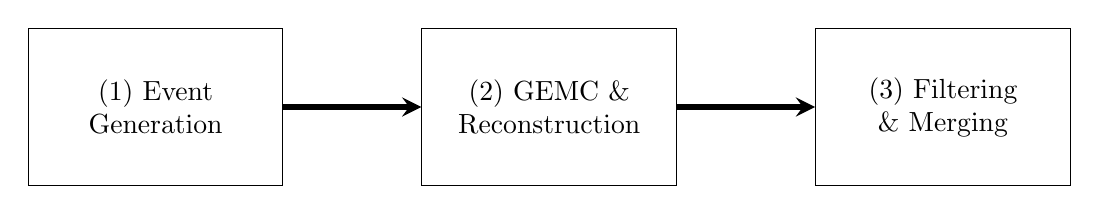
\begin{tikzpicture}[
            box/.style={rectangle, draw, minimum size=2cm, text width=3cm, align=center},
            arrow/.style={->, >=stealth, line width=2pt},
        ]
        
        \node[box] (event) at (0,0) {(1) Event \\ Generation};
        \node[box] (gemc) at (5,0) {(2) GEMC \& \\ Reconstruction};
        \node[box] (filter) at (10,0) {(3) Filtering \& Merging};
        
        \draw[arrow] (event) -- (gemc);
        \draw[arrow] (gemc) -- (filter);
        
        \end{tikzpicture}
        \caption[Event Simulation Pipeline]{Event simulation pipeline. (1) Events are generated using aao\_gen on either MIT Tier 2, MGHPCC, or JLab's SciComp nodes. (2) Events are submitted through the CLAS12 Submission Portal to run on dedicated or idling resources to the GEMC \& CLAS12 event reconstruction suite. (3) Simulated events are returned to JLab's computing nodes, where they are further filtered as discussed in \secref{sec:filtering} and transferred to local computers for analysis.}
        \label{fig:simulation_workflow}
    \end{figure}


    

    \todo{WHERE IS THE JLAB IFARM INFO?}
   
    
    %It includes in addition, a CMS HI simulation and analysis facility, an LHCb Tier-2 computing center, a Hadronic Physics computing center and various smaller contributions. Presently it is located at Bates in Middleton MA.

    %distributed high throughput computing systems - 





    




    
    
    
    %volatile work
    %To cancel all jobs:
    %scancel -u robertej
    
    %To view all jobs:
    %squeue -u robertej

    
    %local of disk utilization statistics: https://clasweb.jlab.org/clas12offline/disk/work/users.html
    




    %is an intercollegiate high-performance computing facility - joint venture between Boston University, Harvard, MIT, Northeastern, and the University of Massachusetts system. - 300 nodes, 10K CPUs, 

 

    
    
    



    
\section{Event Generation}\label{sec:ch3generator}
    The event generators used in this work are based off the MAID unitary isobar model \parencite{Tiator2006MAIDTechniques}, \parencite{Dreschsel1992ThresholdNucleons} which concerns the photo and electroproduction of pions off of nucleons. It originated as an ``\textbf{A}mplitudes \textbf{A}nd \textbf{O}bservables '' (AAO) generator that worked in the resonance regime \parencite{Burkert1991AmplitudesGenerator} and was extended to function at higher W based off theoretical models \parencite{Goloskokov2010AnElectroproduction} and validated on experimental data \parencite{Bedlinskiy2014ExclusiveCLAS} as well as used in recent physics results \parencite{Diehl2022MultidimensionalRegion}. 

There are two generators, ``aao\_norad'', which is a nonradiative generator that creates events with an outgoing electron, proton, and two photons from the decay of the neutral pion, and ``aao\_rad'', which incorporates radiative corrections into the event generation and produces events with an outgoing electron, proton, neutral pion, and radiated photon. These two generators were refactored to function under a larger software package \href{https://github.com/JeffersonLab/aao_gen}{aao\_gen} which provides access to both generators in one system. Sample distributions of the nonradiative generator are shown in \ref{fig:aao_norad_gen}.

    \begin{figure}[H]
        \centering
        \subfloat{\includegraphics[width=0.5\textwidth]{Chapters/Ch3-Simulations/event_generation/pics/Lepton-Hadron_Angle_phi_vs_Proton_theta,_Gen.png}}
        \hfill
        \subfloat{\includegraphics[width=0.5\textwidth]{Chapters/Ch3-Simulations/event_generation/pics/x_B_vs_Q2,_Gen.png}}
        \caption[Generated Event Distributions]{Generated event distributions}\label{fig:aao_norad_gen}
    \end{figure}


The radiative generator builds off the nonradiative generator to include Radiative Corrections (RC). The generator calculates s-peak and p-peak radiative corrections according to the Mo/Tsai scheme \parencite{MO1969RadiativeScattering}. The calculation produces a radiated photon with a distribution as shown in \figref{fig:aao_rad_mom_distribution}. While more realistic than the nonradiative generator, it also takes roughly 100 times as long to produce events, and so in practice both generators are utilized. 


    \begin{figure}
        \centering
        \includegraphics[trim={0 1.25cm 0 2.5cm},clip,width=0.79\textwidth]{Chapters/Ch3-Simulations/event_generation/pics/radiated_photon_momentum.png}
        \caption[aao\_rad radiated photon momentum distribution]{aao\_rad radiated photon momentum distribution. The horizontal axis is the radiated photon momentum, in units of Gev/c.}
        \label{fig:aao_rad_mom_distribution}
    \end{figure}
    
%AAO rad genreates four particles, an electron (PID 11), proton(PID 2212), radiated photon (22), and produced pion  (111)
    

%// Pi0 leptoproduction in Goloskokov-Kroll (GK) model. The code is currently being tested and implemented in PARTONS framework with additional features. If you plan to use this work in a publication, please use and reference the most recent version of PARTONS in http://partons.cea.fr 
\iffalse
% NOTES FROM VALERY KUBEROSKSKY
Andrey Kim and Nick Markov have the pi0 generator. It has my parametrization for W>2 GeV and MAID for W<1.7 GeV.

My model will for sure work for 12 GeV. It actually very close even for the COMPASS pi0 data (180 GeV muon beam).

There is reasonable coincidence between my model and MAID in the point W=1.7 GeV, not ideal but good enough for the MC.

I think actually that my parametrization has to work in the region W<2 GeV but I am not sure that MAID is doing good job due to the absence the experimental data at W~1.7 GeV. 

%FROM ONE OF THE READMES:
***************************************************************************
*      AUTHOR:        V. BURKERT AND Z. LI
*      FIRST VERSION: SUMMER, 1991.  RECENT UPDATE: MAY.1993
* AO IS WRITTEN BASED ON THE ORIGINAL PROGRAM A_AND_O FROM V.BURKERT
* THIS PROGRAM SHOULD BE LINKED TO EITHER QKMC OR QKXM FOR THE CALCULATION
* OF QUARK MODEL.  
* QKMC AND QKXM USE DIFFERENT FORM FACTORS:
* QKMC USES THE TREATMENT OF FOSTER ET. AL.
* QKXM USES THE DIPOLE FORM FACTOR 
* QKMC IS THE DEFAULT CHOICE IN THIS PACKAGE.
* AO CAN BE USED TO EXAM: Q2-DEPENDENCE OF HELICITY AMP. AT RES. POSITION (GO1)
*                         OUTPUT:GDH.TOP: A B CA(A_1/2) CB(A_3/2)
*                         GDH SUM RULE (GO2):OUTPUT GDH.TOP
*                         OBERVABLES  (RETURN):OUTPUT TEST.TOP
**************************************************************************
*           AO.FOR
* AO CONTAINS THE FOLLOWING SUBROUTINES/FUNCTIONS:
* SIGMA--CALCULATES OBSERVABLES
* EPRES--CALCULATES BREIT-WIGNER RESONANCE AMPLITUDES
* EXPA --CALCULATES THE HELICITY AMPLITUTES FROM EXPT (V.BURKERT ORIGINAL)
* BORNT--CALCULATES THE BORN TERM CONTRIBUTIONS
* BACK --CALCULATES BORN AND NON-BORN BACK GROUND TERMSS
* QKMA --CALCULATES THE HELICITY AMPLITUTES FROM QUARK MODEL
* RAMPF --CALCULATES THE Q2-DEPENDENCE OF THE HELICITY AMP. AT RES. POSITIONS
* HAMP --CALCULATES THE ENERGY-DEPENDECE OF THE RESONANCE HELICITY AMPLITUDES
* QKMC --CALCULATES THE COUPLING CONSTANTS FROM QUARK MODEL
************************************************************************
**************************************************************************
* UPDTATED: NOV., 1992
*         * WITH NEW OPTIONS TO TURN THE BORN TERM ON AND OFF
*         * BORN TERM ARE MODIFIED WITH A CUT OFF FACTOR AT HIGHER 
*           ENERGIES (WCM>1.3 GEV)
*         * SOME CORRECTIONS HAVE BEEN MADE TO THE EXPA SUBROUTINE
***************************************************************************  

 %OTHER GENERATOR NOTES:
    For Exclurad we have similar model, in end may have to iterate a few times to improve the model
    Exlclurad specifically for resonance region, theoretically should be correct, input probably needs to be updated, can put Valery’s new parameterization to cover higher range. Should not be a real issue to implement it because same thing was done for AAORad. High q2 cannot be covered because parameterization only goes to CLAS6 range
    FX: the cruicail thing is to fold in the radiative corrections with acceptance and efficiens. Best mothod is to use fast monte carlo


    aao\_rad and aao\_norad are event generators for exclusive pi0 and pi+ channels with/without radiative effects.  They are written in Fortran.  The program was initially developed by Volker Burkert long time ago for the resonance region, then has been evolved for many years and recently extended to DIS region even though lots of things need to be done.  Try this to see whether it works.  
\fi

\iffalse

    \subsection{Nonradiative Generator}
            Include generator plots, specitics of layout
    

    \subsection{Radiative Generator}
     % Include generator plots, specitics of layout, plots showing W cut offs, etc
    %SANGBAEK PG 76 RC
\fi
   

\section{Simulation Pipeline}
    The event generators produce datafiles where each event can be thought of as being represented by 4-vectors (corresponding to the four particles in each event). This represents the (simulated) ground truth of the event. This information must be transformed in a realistic way into the four-momenta typically observed after event reconstruction, data processing, and exclusivity cuts are applied. The most common way to achieve this result is to (1) swim each particle through a physics simulation of the CLAS12 experiment, resulting in simulated detector hits, and (2) pass the simulated detector hit data to reconstruction and analysis algorithms. 

Step (1) is realized through the use of Geometry and Tracking (Geant4) \parencite{Agostinelli2003Geant4aToolkit}, which is a Markov-Chain Monte Carlo (MCMC) software package that simulates the microphyics at each (variable) step along a particle's path through space. This has been implemented for the CLAS12 experiment as a the ``Geant4 Monte Carlo'' (GEMC) software system \parencite{Ungaro2020TheSimulation}, which allows for the simple insertion of CAD models into the Geant4 system, with the basic architecture shown in \ref{fig:gemc_architecture}. 

\begin{figure}[htb]
    \centering
    \includegraphics[width=0.65\textwidth]{Chapters/Ch3-Simulations/simulation_pipeline/pics/gemc_basics.png}
    \caption[GEMC Architecture]{GEMC architecture. Image from \parencite{Ungaro2020TheSimulation}.}
    \label{fig:gemc_architecture}
\end{figure}

Step (2) is straightforward after having been developed as discussed in \chref{Chapter:Experiment}. The distributions from \figref{fig:aao_norad_gen} after passing through the GEMC simulation, CLAS12 reconstruction software, and event selection are shown in \figref{fig:aao_norad_sim}, where the differences between the distributions is indicative of the acceptance cutoffs of the CLAS12 experiment. 


    \begin{figure}[H]
        \centering
        \subfloat[]{\includegraphics[width=0.5\textwidth]{Chapters/Ch3-Simulations/event_generation/pics/x_B_vs_Q2,_rec.png}}
        \hfill
        \subfloat[]{\includegraphics[width=0.5\textwidth]{Chapters/Ch3-Simulations/event_generation/pics/Lepton-Hadron_Angle_phi_vs_Proton_theta,_rec.png}}
        \caption[Reconstructed Event Distributions]{Reconstructed event distributions.}\label{fig:aao_norad_sim}
    \end{figure}

\iffalse
    
    Event generation - fortran and c++ python wrapped
    geant4 docker gemc sysem
    reconstruction from part 2
    
    CLAASana
    
    this should talk about Geant4, GEMC, microphysics MCMC

\fi


    
        


\section{Simulation Enhancements with Normalizing Flows}
    \subsection{Inverse Transforms and Autoregressive Flows}
    Introduce theory of MAFs

\subsection{Exploration of Simulation Speedup with UNMAF}
    Discuss actual work performed





\chapter{Analysis} \label{Chapter:Analysis}
\section{General Analysis Overview}

\section{Data Pre-Processing}
    \subsection{Energy Loss Corrections}
    \subsection{Momentum Corrections}
    \subsection{Simulation:Experiment Resolution Matching}
        \subsubsection{Kinematics Correction of Experimental Data}
        \subsubsection{Smearing Simulated Data}

\section{Particle Identification}

\section{Event Selection}
    \subsection{Rigid Event Selection}
    \subsection{Classifier Based Event Selection}

\section{Luminosity}

\section{Configuration and Kinematics}

\section{Binning}

\section{Acceptance Correction}

\section{Radiative Corrections}

\section{Binning Corrections}

\section{Overall Normalization Corrections}

\section{Error Analysis}



\chapter{Results} \label{Chapter:Results}
\section{General Analysis Overview}

\section{Data Pre-Processing}
    \subsection{Energy Loss Corrections}
    \subsection{Momentum Corrections}
    \subsection{Simulation:Experiment Resolution Matching}
        \subsubsection{Kinematics Correction of Experimental Data}
        \subsubsection{Smearing Simulated Data}

\section{Particle Identification}

\section{Event Selection}
    \subsection{Rigid Event Selection}
    \subsection{Classifier Based Event Selection}

\section{Luminosity}

\section{Configuration and Kinematics}

\section{Binning}

\section{Acceptance Correction}

\section{Radiative Corrections}

\section{Binning Corrections}

\section{Overall Normalization Corrections}

\section{Error Analysis}





Experiment
clas 12 DVMP experiment
Accelerators
Detectors and Recon principles
PID
E ID
Proton ID
Photon Identification
Data processing 

Methods
General analysis technique
event selection
Configuration and kinematics region
Cross section extraction
Simulation pipeline
acceptance correction
Radiative corrections
Monte carlo estimators

Data post processing
energy loss correction for charged particles
electron energy loss
detector regions for proton energy loss correction
details of the two band issue 
proton energy loss correction
biases for higher momentum protons
benehmarks for corrections
Resolution matching 
kinematics correction of experimental data
smearing the simulation data

Results
CLAS12 qality assurance
Event selection revisted
multidimentsional binning
signal yields and acceptance corrections
radiative corrections
normalizatinon and the modified cross section
error analysys
unpolarized corss sections
plarized cross sections
conclusions







%%%%%%%%%%%%%%%%%%%%%%%%%%%%%%%%%%%%%%%%%%%%%%%%%%%% POSTAMBLE %%%%%%%%%%%%%%%%%%%%%%%%%%%%%%%%%%%%%%%%%%%%%%%%%%%%%%%%%%%

\appendix
\bibliography{Postamble/bib/manrefs}
\chapter{}
\section{Full Cross Section Data}
To be completed

\chapter{}
\section{Cross check between Andrey Kim and Bobby Johnston}

As an additional cross check, Bobby calculated a $DV\pi^0P$ beam spin asymmetry and compared to Andrey Kim's results. This check will not comment on any acceptance, luminosity, or virtual photon flux factor calculations, but does validate exclusive event selection criteria. By examining figure \ref{fig:bsa} we can see that agreement is reasonable, especially considering Bobby's calculation does not have sideband subtraction included.

\begin{figure}[hbt]
	\centering
	\includegraphics[width=0.75\linewidth]{Postamble/appb_pics/BSA.png}
	
	
	\caption{Overlay comparison of Andrey Kim's results (black datapoints, red fit line) and Bobby's results (red datapoints, orange fit line).}
	\label{fig:bsa}
\end{figure}


\end{document}
